\documentclass[a4paper,
fontsize=11pt,
%headings=small,
oneside,
numbers=noperiodatend,
parskip=half-,
bibliography=totoc,
final
]{scrartcl}

\usepackage{synttree}
\usepackage{graphicx}
\setkeys{Gin}{width=.4\textwidth} %default pics size

\graphicspath{{./plots/}}
\usepackage[ngerman]{babel}
\usepackage[T1]{fontenc}
%\usepackage{amsmath}
\usepackage[utf8x]{inputenc}
\usepackage [hyphens]{url}
\usepackage{booktabs} 
\usepackage[left=2.4cm,right=2.4cm,top=2.3cm,bottom=2cm,includeheadfoot]{geometry}
\usepackage{eurosym}
\usepackage{multirow}
\usepackage[ngerman]{varioref}
\setcapindent{1em}
\renewcommand{\labelitemi}{--}
\usepackage{paralist}
\usepackage{pdfpages}
\usepackage{lscape}
\usepackage{float}
\usepackage{acronym}
\usepackage{eurosym}
\usepackage[babel]{csquotes}
\usepackage{longtable,lscape}
\usepackage{mathpazo}
\usepackage[normalem]{ulem} %emphasize weiterhin kursiv
\usepackage[flushmargin,ragged]{footmisc} % left align footnote
\usepackage{ccicons} 
\setcapindent{0pt} % no indentation in captions

%%%% fancy LIBREAS URL color 
\usepackage{xcolor}
\definecolor{libreas}{RGB}{112,0,0}

\usepackage{listings}

\urlstyle{same}  % don't use monospace font for urls

\usepackage[fleqn]{amsmath}

%adjust fontsize for part

\usepackage{sectsty}
\partfont{\large}

%Das BibTeX-Zeichen mit \BibTeX setzen:
\def\symbol#1{\char #1\relax}
\def\bsl{{\tt\symbol{'134}}}
\def\BibTeX{{\rm B\kern-.05em{\sc i\kern-.025em b}\kern-.08em
    T\kern-.1667em\lower.7ex\hbox{E}\kern-.125emX}}

\usepackage{fancyhdr}
\fancyhf{}
\pagestyle{fancyplain}
\fancyhead[R]{\thepage}

% make sure bookmarks are created eventough sections are not numbered!
 %uncommend if sections are numbered (bookmarks created by default)
\makeatletter
\renewcommand\@seccntformat[1]{}
\makeatother


\usepackage{hyperxmp}
\usepackage[colorlinks, linkcolor=black,citecolor=black, urlcolor=libreas,
breaklinks= true,bookmarks=true,bookmarksopen=true]{hyperref}
\usepackage{breakurl}

%meta
%meta

\fancyhead[L]{M. Voigt, S. Dittmann\\ %author
LIBREAS. Library Ideas, 35 (2019). % journal, issue, volume.
\href{http://nbn-resolving.de/}
{}} % urn 
% recommended use
%\href{http://nbn-resolving.de/}{\color{black}{urn:nbn:de...}}
\fancyhead[R]{\thepage} %page number
\fancyfoot[L] {\ccLogo \ccAttribution\ \href{https://creativecommons.org/licenses/by/4.0/}{\color{black}Creative Commons BY 4.0}}  %licence
\fancyfoot[R] {ISSN: 1860-7950}

\title{\LARGE{Zweitveröffentlichungsservice der TU Berlin – Automatisierungsmöglichkeiten für den Workflow}}% title
\author{Michaela Voigt, Sebastian Dittmann} % author

\setcounter{page}{1}

\hypersetup{%
      pdftitle={Zweitveröffentlichungsservice der TU Berlin – Automatisierungsmöglichkeiten für den Workflow},
      pdfauthor={Michaela Voigt, Sebastian Dittmann},
      pdfcopyright={CC BY 4.0 International},
      pdfsubject={LIBREAS. Library Ideas, 35 (2019).},
      pdfkeywords={Open Access, Grüner Weg, Zweitveröffentlichung, Service, Workflow, TU Berlin, OpenRefine},
      pdflicenseurl={https://creativecommons.org/licenses/by/4.0/},
      pdfcontacturl={http://libreas.eu},
      baseurl={http://libreas.eu},
      pdflang={de},
      pdfmetalang={de}
     }



\date{}
\begin{document}

\maketitle
\thispagestyle{fancyplain} 

%abstracts
\begin{abstract}
\noindent\textbf{Kurzfassung}: Der Artikel stellt den mithilfe von OpenRefine
teilautomatisierten Workflow des Zweitveröffentlichungsservices der
Technischen Universität Berlin vor: Es werden Hintergründe und
Abwägungen, die einzelnen Schritte im Workflow und Möglichkeiten zur
Nachnutzung der erarbeiteten Materialien beschrieben und diskutiert.
\end{abstract}

%body
\hypertarget{hintergrund}{%
\section{Hintergrund}\label{hintergrund}}

Anfang 2015 hat die Universitätsbibliothek der TU Berlin den
\enquote{Zweitveröffentlichungsservice} für TU-Angehörige eingeführt. Er
sollte ein praktischer Service sein, um TU-Angehörige dabei zu
unterstützen, ihre Publikationen über den Grünen Weg frei zugänglich zu
machen -- und damit die allgemeine Beratung zu Open Access (OA)
ergänzen. Einen zentralen Publikationsfonds zur Unterstützung für den
Goldenen Weg gab es zu dem Zeitpunkt noch nicht. Unser Open-Access-Team
wurde gerade aufgebaut -- mit zunächst einer Mitarbeiterin, wobei der
Zweitveröffentlichungsservice nur ein Aufgabenfeld unter vielen war. Das
Angebot war niedrigschwellig formuliert: \enquote{Schicken Sie uns Ihre
Publikationsliste, wir prüfen die rechtlichen Voraussetzungen für eine
Zweitveröffentlichung und übernehmen das Einstellen der zulässigen
Beiträge in DepositOnce, dem institutionellen Repositorium der TU
Berlin.} Dieses Angebot richtete sich an Einzelpersonen, Lehrstühle (im
TU-Sprech \enquote{Fachgebiete}) und andere Arbeitsgruppen.

Das klingt einfach; schnell stellte sich jedoch heraus, welche Hürden es
im Alltag zu überwinden gilt:

\begin{enumerate}
\def\labelenumi{\arabic{enumi}.}
\item
  Publikationsdaten: An der TU Berlin gibt es keine öffentliche
  Hochschulbibliografie und auch keine interne Bibliografie mit
  Exportfunktionen in gängigen Formaten. Die Erfassung von
  Publikationsleistungen erfolgt in einer TU-internen Datenbank, die
  durch die Forschungsabteilung betreut wird und auf die
  Bibliotheksmitarbeiter*innen nicht zugreifen können.
\item
  Publikationsliste: Wir hatten anfänglich gehofft, dass uns Autor*innen
  ihre Listen in einem strukturierten Format -- idealerweise als RIS-
  oder Bibtex-Datei -- zusenden würden. Dies wurde aber nicht zur
  Voraussetzung gemacht, denn das Motto war \enquote{easy to do business
  with}, die Hürden zur Beteiligung sollten also so gering wie möglich
  sein. Strukturierte bibliografische Daten haben wir nur in
  Ausnahmefällen erhalten -- stattdessen PDF- oder Word-Dateien, Links
  zu persönlichen Homepages oder TU-Webseiten. Die darin enthaltenen
  bibliografischen Einträge waren heterogen: Wir fanden unterschiedliche
  Schreibweisen von Autor*innen (Umlaute, \enquote{et al.}, Abkürzungen)
  und Zeitschriften- oder Buchtiteln (insbesondere Abkürzungen,
  uneinheitliche Angaben trotz gleicher Zeitschrift) vor. DOIs wurden
  nur zum Teil angegeben; Links waren häufig als nicht-persistente
  Direktlinks zur Onlineversion enthalten. Angaben zu Verlagen gab es
  mitunter, ISSN oder ISBN hingegen nicht. Der Aufwand für die
  Erstellung einer tabellarischen Übersicht, anhand derer eine
  Rechteprüfung strukturiert durchgeführt und der Fortschritt der
  Bearbeitung pro Titel überwacht werden kann, war nicht unerheblich.
\item
  Interesse am Service: Der neue Service wurde über verschiedene Kanäle
  der Bibliothek beworben (unter anderem Webseite,
  Open-Access-Workshops, Beratungsgespräche für Autor*innen des
  Universitätsverlags, Information über Fachreferent*innen). Auf
  Interessierte mussten wir nicht lange warten; die ersten eingereichten
  Listen konnten wir vergleichsweise zügig bearbeiten. Schon Anfang 2016
  wurde deutlich, dass die Nachfrage aufseiten der TU-Angehörigen die
  personellen Kapazitäten im Open-Access-Team überschritt. Eine
  Reduktion der Bearbeitungszeit konnte auch 2017 trotz neuer
  Mitarbeiter*innen im Team nicht erreicht werden. Spätestens 2018 war
  klar, dass das Angebot als solches zwar zuvorkommend formuliert ist,
  aber in der Praxis nicht den Ansprüchen gerecht werden kann (weder
  denen der Autor*innen noch den eigenen).
\end{enumerate}

Der Grüne Weg ist ein Mengenproblem, insbesondere wenn den Autor*innen
so viele Aspekte wie möglich abgenommen werden sollen (neben der
eigentlichen Rechteprüfung auch Anfragen bei Verlagen, Erfassung von
Metadaten im Repositorium und Aufbereitung von Dateien). Dass es einen
so umfangreichen Service braucht, um den Anteil der über den Grünen Weg
frei verfügbaren Publikationen zu fördern, schien uns durch die Tatsache
offensichtlich, dass an der TU Berlin bereits seit Ende der 1990er ein
Repositorium betrieben wird, welches jedoch nie in nennenswertem Umfang
durch Autor*innen für Zweitveröffentlichungen eigeninitiativ genutzt
wurde. 2018 haben wir daher begonnen, das Automatisierungspotential
auszuloten.

Wie begegnen andere Bibliotheken dem Wunsch nach mehr grünem Open Access
und dem \enquote{Mengenproblem}? Blasetti et al.~(2019) stellen
verschiedene Rechtsgrundlagen für Zweitveröffentlichungen vor und
diskutieren Fragen, die sich rund um das Angebot eines regulären
bibliothekarischen Zweitveröffentlichungsservices stellen können. Der
Beitrag gibt Anregungen zur praktischen Umsetzung in Form von
Checklisten und diskutiert Optionen für die Automatisierung -- er
präsentiert jedoch kein festes Verfahren, das Einrichtungen lokal
adaptieren können.

Galvan (2016) setzt auf OpenRefine\footnote{OpenRefine ist eine
  plattformunabhängige Open-Source-Software und laut Selbstbeschreibung
  ein \enquote{powerful tool for working with messy data} (siehe
  \url{http://openrefine.org/}). OpenRefine ermöglicht unter anderem die
  Bereinigung, (Format-)Transformation und Aggregation von Daten.}, um
auf Basis von bibliografischen Daten (exportiert etwa aus
Fachdatenbanken) die Schnittstelle von SHERPA/RoMEO abzufragen. In einer
Schritt-für-Schritt-Anleitung zeigt sie, wie man mit OpenRefine einzelne
XML-Felder in verschiedene Spalten überführen kann, um nicht
SHERPA/RoMEO-Einträge pro Zeitschrift einzeln im Browser aufzurufen und
Angaben zu Verlagspolicies zu extrahieren. Rele \& Young (2017)
beschreiben die Automatisierung des Workflows für die Loyola Marymount
University. Ausgangspunkt sind Literaturlisten von Fakultätsangehörigen
oder Exporte aus Web of Science, die mithilfe von Google Spreadsheets
aufbereitet und mit Daten aus SHERPA/RoMEO angereichert werden. Tobias
(2018) beschreibt, wie die Integration von Hochschulbibliografie und
Repositorium am KIT Karlsruhe umgesetzt wurde, um
Zweitveröffentlichungsworkflows zu skalieren und das Verfahren für
Autor*innen und Mitarbeiter*innen der Bibliothek leicht, überschaubar
und im Alltag umsetzbar zu gestalten.

Der vorliegende Artikel stellt den teilautomatisierten Workflow des
Zweitveröffentlichungsservices an der TU Berlin vor, der seit Ende 2018
im produktiven Einsatz ist und kontinuierlich weiterentwickelt wird. Die
eingesetzten Skripte und eine ausführliche Dokumentation sind auf GitHub
verfügbar: \url{https://github.com/tuub/oagreenservice}. Wir hoffen,
dass diese Materialien an anderen Einrichtungen genutzt werden können,
um den Workflow des Zweitveröffentlichungsservices zu verbessern und
Teilschritte zu automatisieren.

\hypertarget{vorgehen}{%
\section{Vorgehen}\label{vorgehen}}

Der Workflow wurde anhand der folgenden Prämissen und lokalen
Voraussetzungen an der Universitätsbibliothek der TU Berlin entwickelt:

\begin{itemize}
\item
  Mitarbeiter*innen: Das Open-Access-Team der Universitätsbibliothek
  besteht aus mehreren Personen mit vielfältigen Aufgaben und
  unterschiedlichen (technischen) Fertigkeiten. Häufig bekommen wir
  temporäre Unterstützung durch FaMI-Auszubildende, Praktikant*innen
  oder Referendar*innen, die in der eher kurzen Zeit bei uns nicht in
  alle Schritte (Rechteprüfung, Kontakt mit Autor*innen und ggf.
  Verlagen, Aufbereitung von Dateien, Metadateneingabe) eingearbeitet,
  jedoch für einzelne Arbeiten eingebunden werden können.
\item
  (Technische) Vorkenntnisse: Im Team gibt es bereits umfangreiche
  Erfahrung im Umgang mit OpenRefine, sowohl für die Transformation von
  Daten als auch für die Abfrage von Webschnittstellen. Erweiterte
  Programmierkenntnisse sind nur bei einem (befristet beschäftigten)
  Mitarbeiter vorhanden.
\item
  Repositorium: Das institutionelle Repositorium DepositOnce basiert auf
  DSpace 6. Aktuell gibt es auf DepositOnce keine Möglichkeit, Metadaten
  über eine direkte Anbindung von Crossref zu importieren. Neue
  Datensätze können entweder durch manuelle Eingabe in einem Webformular
  oder den Import von CSV-Dateien angelegt werden.
\item
  Schnittstellen: Es gibt zahlreiche (freie) Webschnittstellen, die für
  einen Zweitveröffentlichungsservice relevant sind -- etwa von
  Crossref, SHERPA/RoMEO, Unpaywall und Crosscite.
\end{itemize}

Vor diesem Hintergrund bietet es sich an, den Workflow so zu gliedern,
dass die Bearbeitung umfangreicher Publikationslisten arbeitsteilig,
effizient und unter Berücksichtigung jeweiliger Interessen und
Vorkenntnisse der eingebundenen Personen gestaltet werden kann.

\hypertarget{datenquellen}{%
\subsection{Datenquellen}\label{datenquellen}}

Für die Aggregation von Daten zu Publikationen kommen primär folgende
Quellen zum Beispiel für die Nachnutzung bibliografischer Daten, Angaben
zum Open-Access-Status, Lizenzierung oder Verlagspolicies (alphabetische
Sortierung) zum Einsatz:

\textbf{Crosscite} ist ein gemeinsamer Service der vier
DOI-Registrierungsagenturen Crossref, DataCite, mEDRA und ISTIC.
Mithilfe von Crosscite können bibliografische Daten in verschiedenen
Datenformaten (unter anderem RIS, Bibtex, JSON, XML) oder als
formatierte Zitation abgerufen werden, wobei zahlreiche Zitierstile
sowie Gebietsschemata (Sprache und Land) auswählbar sind. Eine
Dokumentation des Dienstes ist online verfügbar; auf der Webseite können
über eine grafische Oberfläche Zitationen auf Basis von DOIs erzeugt
werden. Mit der Nutzung von Crosscite kann der Formatierungsaufwand für
eine einheitliche Zitation reduziert werden, die entweder in den
Metadaten und/oder einem dem Volltext vorangestellten Titelblatt
eingebunden werden soll. \footnote{Crosscite: Webseite siehe
  \url{https://crosscite.org/}, Dokumentation siehe
  \url{https://crosscite.org/docs.html}}

\textbf{Crossref}: Für die überwiegende Mehrzahl der Publikationen, für
die Autor*innen eine Zweitveröffentlichung wünschen, wird eine DOI über
Crossref registriert. Um die von den Verlagen registrierten Metadaten
abzufragen, kann die REST-Schnittstelle genutzt werden.\footnote{Crossref:
  ausführliche Dokumentation zur Schnittstelle siehe
  \url{http://api.crossref.org/}} Die Nutzung ist kostenfrei, eine
Registrierung ist nicht erforderlich. Durch Abfrage einer DOI können
unter anderem Angaben zu Autor*innen, Titel, Journal bzw. Buch, ISSN und
ISBN, Band und Heft, Seitenzahlen oder zur Lizenz der Verlagsversion
bezogen werden.

\textbf{DepositOnce} ist das institutionelle Repositorium der TU Berlin.
Autor*innen reichen häufig vollständige Publikationslisten ein; unter
Umständen sind einzelne Beiträge bereits auf DepositOnce verfügbar. Um
Dubletten im Repositorium sowie unnötige Schritte bei der Bearbeitung zu
vermeiden, werden Verlags-DOI und Titel des Beitrags an eine interne
Schnittstelle von DepositOnce übermittelt und potenzielle Dubletten
markiert.

\textbf{DOI-Resolver}: Mitunter liefert die Crossref-Abfrage keine Daten
zurück; dies kann verschiedene Gründe haben: Die DOI wurde über eine
andere DOI-Agentur registriert; die DOI wurde nicht (korrekt) vom Verlag
registriert; die DOI ist syntaktisch nicht korrekt. Um die Fehlersuche
zu erleichtern, bietet sich eine Anfrage an den globalen DOI-Resolver
\texttt{https://doi.org/doiRA/\\\$DOI} an: Wurde die angefragte DOI registriert,
wird die jeweilige DOI-Agentur ausgegeben; andernfalls gibt der Resolver
Fehlermeldungen (zum Beispiel \enquote{DOI does not exist} oder
\enquote{Invalid DOI}) zurück. Dies lässt sich am einfachsten an einem
Beispiel veranschaulichen:

\begin{itemize}
\item
  unvollständige DOI: \url{http://doi.org/doiRA/10.17161/jcel.v2i1.716}
  mit Angabe \texttt{status: "DOI does not exist"}
\item
  valide DOI: \url{http://doi.org/doiRA/10.17161/jcel.v2i1.7162} mit
  Angabe \texttt{RA: "Crossref"}
\end{itemize}

\textbf{OA-EZB-Schnittstelle:} Im Rahmen von Allianz- und
Nationallizenzen wurden Open-Access-Rechte für die lizenznehmenden
Institutionen verhandelt, das heißt Verlage räumen mitunter den
Institutionen direkt Rechte zur Zweitveröffentlichung ein. Diese Rechte
gehen in der Regel über die vom Verlag im Rahmen der allgemeinen Policy
eingeräumten Rechte für Autor*innen hinaus. Bislang gestaltete sich die
Recherche danach, ob für einen bestimmten Artikel Open-Access-Rechte
vorliegen, als aufwändig (vgl. Thomas \& Stadler (2016), Voigt (2016)).
Das DFG-geförderte Projekt OA-EZB hatte zum Ziel, Angaben zu diesen
besonderen Open-Access-Rechten in der Elektronischen
Zeitschriftenbibliothek (EZB) zu verankern und maschinell abfragbar zu
machen. Resultat ist die OA-EZB-Schnittstelle, welche die in der EZB
hinterlegten Open-Access-Rechte zur Veröffentlichung von Volltexten
gemäß Allianz-, National- oder Konsortiallizenzen zur Verfügung stellt
und für die keine Registrierung erforderlich ist. Um die OA-Berechtigung
für die eigene Institution zu ermitteln, ist die EZB-Kennung anzugeben.
Die Abfrage kann auf Artikel- oder Zeitschriftenebene erfolgen; Daten
werden in den Formaten JSON oder XML zurückgegeben.\footnote{OA-EZB:
  Dokumentation zur Schnittstelle siehe
  \url{https://ezb.ur.de/services/oa-ezb}}

\textbf{SHERPA/RoMEO}: Zahlreiche Verlage stellen auf ihren Webseiten
Informationen darüber bereit, ob beziehungsweise zu welchen Bedingungen
eine Zweitveröffentlichung möglich ist. Die Datenbank SHERPA/RoMEO
bietet einen übersichtlichen Einstieg in die unterschiedlichen
Richtlinien der einzelnen Verlage. Sie ordnet zudem die Policies ein: Je
nach Manuskriptversion (Preprint, Postprint, Verlagsversion) wird
unterschieden nach \enquote{gestattet}, \enquote{nicht gestattet} oder
\enquote{unbekannt}. Zudem werden im Bereich \enquote{General
Conditions} die zu beachtenden Bedingungen aufgeführt. Neben
bibliografischen Angaben zur Zeitschrift werden Links zur Verlagspolicy
bzw. zum Standardvertrag gelistet. Alle Angaben zu Verlagspolicies, die
über die Webseite von SHERPA/RoMEO recherchierbar sind, können auch über
die REST-Schnittstelle abgefragt werden. Dafür ist eine Registrierung
erforderlich, bei der ein sogenannter API-key zugeteilt wird -- ein
Schlüssel zur Authentifizierung, dessen Angabe bei der Abfrage
verpflichtend ist. Daten werden im XML-Format ausgeliefert. Zwar ist
auch eine Suche nach Zeitschriftentitel oder Verlagsnamen über die
Schnittstelle möglich; am verlässlichsten sind allerdings Abfragen über
die ISSN, um eine Zuordnung zur falschen Zeitschrift zu vermeiden.
\footnote{SHERPA/RoMEO: Webseite siehe
  \url{http://www.sherpa.ac.uk/romeo/}, Schnittstelle siehe
  \url{http://www.sherpa.ac.uk/romeo/api29.php}, API-Dokumentation siehe
  \url{http://www.sherpa.ac.uk/romeo/apimanual}}

\textbf{Unpaywall} ist ein Webservice, um auf Basis einer DOI den
Open-Access-Status einer Publikation zu ermitteln: Wurde ein Artikel in
einer OA-Zeitschrift publiziert? Steht die Verlagsversion unter einer
freien Lizenz? Gibt es bereits eine frei zugängliche Version eines
Artikels über ein Repositorium? Diese und ähnliche Fragen können
mithilfe von Unpaywall-Daten beantwortet werden. 100.000 Abfragen am Tag
an die REST-Schnittstelle sind frei; eine Registrierung ist nicht
erforderlich, jedoch soll bei jeder Abfrage die E-Mail-Adresse
übermittelt werden. Eine Dokumentation der Unpaywall-Datenfelder ist
online verfügbar.\footnote{Unpaywall: Schnittstelle siehe
  \url{https://unpaywall.org/products/api}, Dokumentation Datenfelder
  siehe \url{https://unpaywall.org/data-format}}

Folgenden Datenquellen nutzen wir zusätzlich, um Abstracts und Keywords
zu den einzelnen Publikationen zu beziehen -- für den Workflow spielen
sie aufgrund der bisher geringen \enquote{Erfolgsquote} allerdings noch
eine untergeordnete Rolle:

\textbf{arXiv} ist ein Preprint-Server mit fachlichem Schwerpunkt in den
Bereichen Physik, Mathematik, Informatik, Statistik, Finanzmathematik
und Biologie. arXiv stellt Daten über eine Schnittstelle zur Verfügung,
für die keinerlei Registrierung oder Authentifizierung erforderlich
ist.\footnote{arXiv: Webseite siehe \url{https://arxiv.org/},
  Dokumentation zur Schnittstelle siehe \url{https://arxiv.org/help/api}}

\textbf{BASE:} Die wissenschaftliche Suchmaschine BASE aggregiert
bibliografische Daten verschiedener Services auf Basis der jeweiligen
OAI-Schnittstelle (Repositorien, Open-Access-Zeitschriften,
Forschungsinformationssysteme, Digitale Sammlungen und so weiter). Um
die Schnittstelle nutzen zu können, muss die IP-Adresse freigeschaltet
werden.\footnote{BASE: Webseite siehe \url{https://www.base-search.net},
  Dokumentation zur Schnittstelle siehe
  \url{https://www.base-search.net/about/download/base_interface.pdf}}

\textbf{CORE} aggregiert Metadaten und Volltexte von Repositorien und
Journalen auf Basis der jeweiligen OAI-Schnittstellen. Bibliografische
Daten stellt CORE auch über eine Schnittstelle zur Verfügung. Um diese
abfragen zu können, muss ein API-key registriert werden, dessen Angabe
bei der Abfrage verpflichtend ist.\footnote{CORE: Webseite siehe
  \url{https://core.ac.uk}, Dokumentation zur Schnittstelle siehe
  \url{https://core.ac.uk/documentation/api}}

\textbf{PubMed} ist die einschlägige Fach- und Literaturdatenbank für
Publikationen aus dem Bereich (Bio-)Medizin und wird betrieben von der
US-amerikanischen National Library of Medicine. PubMed stellt
verschiedene Schnittstellen zur Verfügung, um auf Basis einer
sogenannten Pub\-Med-ID oder einer DOI Metadaten abzufragen; es liegt
jeweils eine ausführliche Dokumentation vor.\footnote{PubMed: Webseite
  siehe \url{https://www.ncbi.nlm.nih.gov/pubmed/}, Übersicht verfügbare
  Schnittstellen siehe
  \url{https://www.ncbi.nlm.nih.gov/home/develop/api/}}

\textbf{Springer:} Der Wissenschaftsverlag Springer stellt für eigene
Publikationen bibliografische Daten über verschiedene Schnittstellen zur
Verfügung. Über die \enquote{Springer Nature Metadata API} etwa können
Metadaten zu Zeitschriftenartikeln, Buchkapiteln et cetera abgefragt
werden. Dafür muss ein API-key registriert werden, dessen Angabe bei der
Abfrage verpflichtend ist. Wir gleichen zunächst DOI-Präfixe mit Angaben
von Crossref ab, um nur für die von Springer verwalteten DOIs Abfragen
an die Springer-Schnittstelle zu stellen.\footnote{Springer:
  Dokumentation zur Schnittstelle siehe Verfügung
  \url{https://dev.springernature.com/}}

\hypertarget{schritte-im-workflow}{%
\subsection{Schritte im Workflow}\label{schritte-im-workflow}}

Der Workflow ist in verschiedene Module unterteilt (siehe Abbildung),
für deren Bearbeitung mehrfach zwischen OpenRefine (für die Abfrage von
Schnittstellen und Transformation von Metadaten) und Excel (für die
manuelle Datenaufbereitung) gewechselt wird. Für jedes Modul, das in
OpenRefine bearbeitet wird, ist ein separates Projekt anzulegen. Nach
Abschluss der Arbeiten in OpenRefine wird das Projekt als Excel-Datei
exportiert.

Für die Projektverwaltung wird Trello\footnote{Trello siehe
  \url{https://trello.com}} genutzt, sowohl für die Übersicht über
ausstehende Projekte als auch zur Überwachung des Fortgangs und offener
Aufgaben in einzelnen Projekten. Projekt meint dabei eine
Publikationsliste mit mehr als fünf Beiträgen. Einzelne Publikationen
werden als solche behandelt; für diese würde der unten beschriebene
Ablauf keinen Zeitgewinn bedeuten.

Die Ablage von Dateien erfolgt im lokalen Laufwerk der Abteilung;
jegliche Kommunikation mit Autor*innen und gegebenenfalls mit Verlagen
erfolgt über die Teammailbox des Open-Access-Teams.

Der im Folgenden beschriebene Workflow ist nicht unbedingt linear; etwa
die Dateibeschaffung und Metadatenkontrolle können parallel ablaufen. Er
wird hier überblicksartig beschrieben -- weitere Details sind dem
GitHub-Repository zu entnehmen.

\begin{figure}
\centering
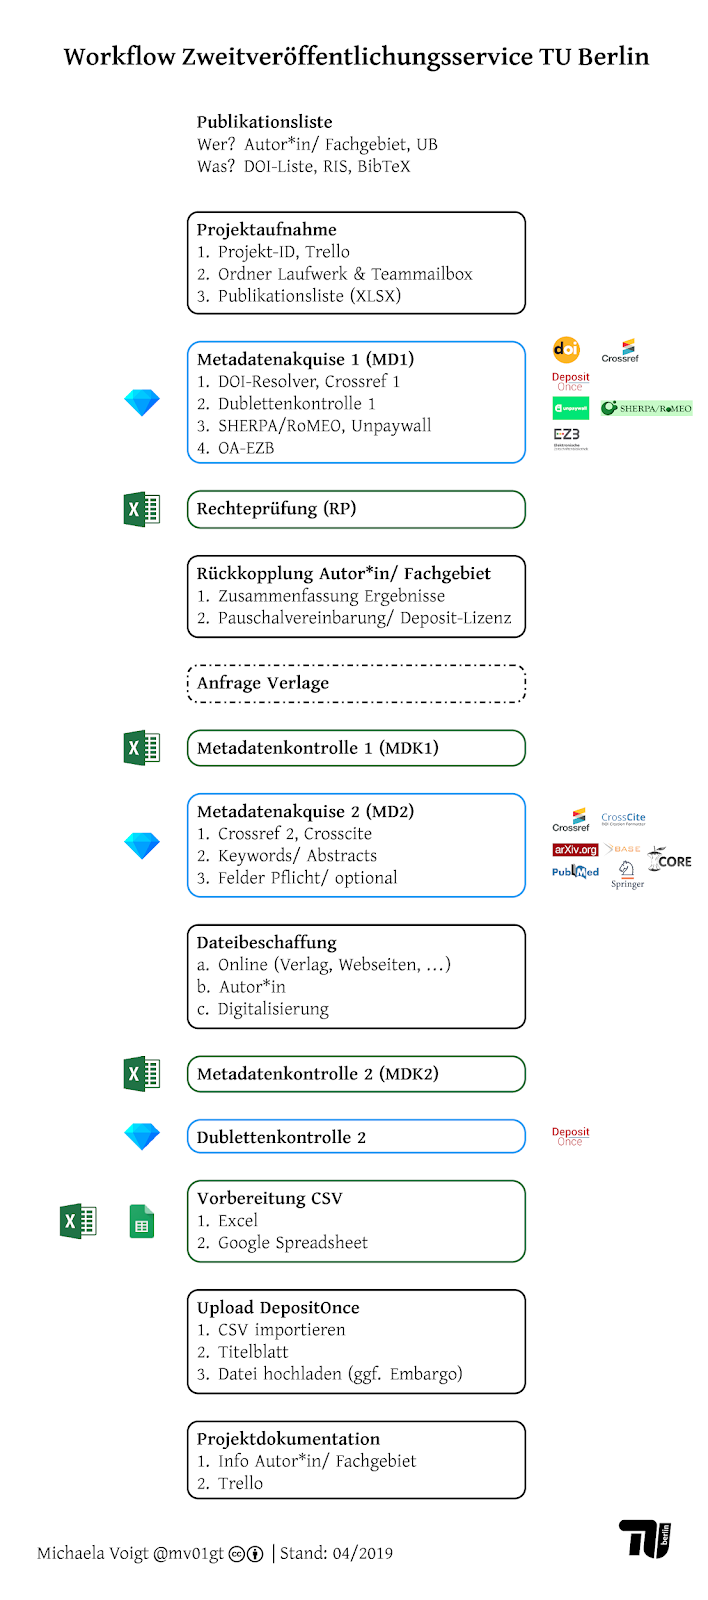
\includegraphics[width=9.3 cm]{img/fig1.png}
\caption{Überblick Workflow Zweitveröffentlichungsservice TU Berlin}
\end{figure}

\hypertarget{projektaufnahme}{%
\subsubsection{Projektaufnahme}\label{projektaufnahme}}

Autor*innen, die eine Zweitveröffentlichung wünschen, sind aufgefordert,
ihre Publikationen in Form einer Liste von DOIs zu übermitteln. Dies
kann in jedem Format erfolgen (direkt einkopiert in eine E-Mail, als
Word- oder Excel-Datei); maßgeblich ist lediglich, dass sich die DOIs
direkt oder ohne Aufwand als Zeichenfolge extrahieren lassen.
TU-Angehörige, die mit Literaturverwaltungsprogrammen arbeiten,
übermitteln ihre Liste erfreulicherweise häufig im Bibtex-Format. Für
Beiträge ohne DOI wird die Abgabe im Bibtex- oder RIS-Format verlangt.

Die Projektaufnahme umfasst die Vergabe einer übergeordneten Projekt-ID
und das Anlegen einer Projektübersicht in Trello, das Anlegen
entsprechender Ordner im lokalen Laufwerk und in der Teammailbox sowie
die Vorbereitung der Publikationsliste im Tabellenformat. Diese Liste
muss einem bestimmten Muster entsprechen; im einfachsten Fall sind
lediglich zwei Spalten ausgefüllt (\enquote{Projekt Nr.} und
\enquote{DOI}). Bibtex- oder RIS-Dateien werden vorab mithilfe von
Citavi in ein Tabellenformat überführt.

\hypertarget{metadatenakquise-1}{%
\subsubsection{Metadatenakquise 1}\label{metadatenakquise-1}}

Liegt die Publikationsliste im erforderlichen Format vor, kommen
erstmals OpenRefine-Skripte zum Einsatz, um Daten aus diversen Quellen
zu aggregieren: Es wird zunächst auf Basis der DOI der globale
DOI-Resolver abgefragt, um zu überprüfen, ob die DOI syntaktisch korrekt
ist und Metadaten bei Crossref registriert wurden. Daran schließt die
Abfrage von Crossref an, um ein Grundset an Metadaten zu akquirieren,
das für die Rechteprüfung erforderlich ist. Um einerseits effizient bei
der Rechteprüfung vorzugehen und andererseits Dubletten im Repositorium
zu verhindern, wird im Anschluss geprüft, ob die gelisteten
Publikationen bereits auf DepositOnce verfügbar sind. Zur Unterstützung
der Rechteprüfung werden Angaben zu Verlagspolicies von SHERPA/RoMEO,
zum aktuellen Open-Access-Status von Unpaywall und zu etwaigen
Open-Access-Rechten aus Allianz- oder Nationallizenzen von OA-EZB
abgefragt. In OpenRefine sind an dieser Stelle lediglich die
entsprechenden Skripte auszuführen; anschließend wird das Projekt als
Excel-Datei exportiert.

\hypertarget{rechtepruxfcfung}{%
\subsubsection{Rechteprüfung}\label{rechtepruxfcfung}}

Die eigentliche Rechteprüfung erfolgt in Excel. Mitunter können für
einen Beitrag mehrere Rechtsgrundlagen für eine Zweitveröffentlichung
vorliegen. Ziel ist die Identifikation der bestmöglichen
Manuskriptversion (Preprint, Postprint oder Verlagsversion) zu den
günstigsten Bedingungen (Embargofrist und andere Auflagen der Verlage).
Daher werden die Rechtsgrundlagen verschieden priorisiert und die
Anwendbarkeit in der folgenden Reihenfolge geprüft:

\begin{itemize}
\item
  Vorliegen einer Creative-Commons-Lizenz
\item
  Open-Access-Rechte aus Allianz- oder Nationallizenzen
\item
  Gesetzlich verankertes Zweitveröffentlichungsrecht nach § 38 (4)
  Urheberrechtsgesetz (bei Zeitschriftenartikeln ab 2014)
\item
  Verlagspolicy
\end{itemize}

Kann die Rechtesituation nicht eindeutig bestimmt werden, wird dies
dokumentiert und wenn möglich werden Kontaktdaten für eine spätere
Anfrage an den Verlag erfasst.

\hypertarget{ruxfcckkopplung-autorin}{%
\subsubsection{Rückkopplung Autor*in}\label{ruxfcckkopplung-autorin}}

Nach der Rechteprüfung erfolgt erstmalig nach Projektannahme die
Rückkopplung mit den Autor*innen: Es werden die Ergebnisse der
Rechteprüfung überblicksartig zusammengefasst und Informationen zum
weiteren Vorgehen gegeben. Die Autor*innen werden aufgefordert, eine
schriftliche Einverständniserklärung für die Zweitveröffentlichung
einzureichen -- diese dient als Nachweis, dass die Zweitveröffentlichung
auf Wunsch der Autor*innen erfolgt, denn der Upload im Repositorium und
damit die Zustimmung zur Deposit-Lizenz wird durch das Open-Access-Team
vorgenommen.\footnote{Für Zweitveröffentlichungen übernimmt die
  Universitätsbibliothek die rechtliche Verantwortung und stellt
  Autor*innen von der Haftung frei. Autor*innen sind lediglich
  aufgefordert, Koautor*innen über die geplante Zweitveröffentlichung zu
  informieren beziehungsweise informell deren Zustimmung einzuholen. Ein
  Nachweis über das Einverständnis der Koautor*innen wird vonseiten der
  Universitätsbibliothek nicht eingefordert.} In der Regel
unterschreiben die Autor*innen eine pauschale Einverständniserklärung,
so dass für zukünftige Publikationen kein weiteres Formular einzureichen
ist.\footnote{Pauschale Einverständniserklärung oder
  Pauschalvereinbarung meint eine Deposit-Lizenz, mit der Autor*innen
  pauschal für alle TU-affiliierten Publikationen der
  Universitätsbibliothek das einfache Recht zur Zweitveröffentlichung
  auf dem Repositorium übertragen. Diese Lizenz enthält den Hinweis,
  dass eine Zweitveröffentlichung nur nach einer entsprechenden
  Rechteprüfung durchgeführt wird und ein Kündigungsrecht für die
  Autor*innen.} Auf Wunsch kann die Deposit-Lizenz jedoch auch auf
Einzelfallbasis eingereicht werden.

\hypertarget{anfrage-verlage}{%
\subsubsection{Anfrage Verlage}\label{anfrage-verlage}}

Verlage werden angeschrieben, um die für eine Zweitveröffentlichung
erforderlichen Rechte einzuholen -- außer die Autor*in hat explizit den
Wunsch geäußert, dass Verlage nicht kontaktiert werden. Dabei wird die
Nutzung der Verlagsversion angefragt. Der Fortschritt der Anfrage ist in
der Excel-Datei zu dokumentieren. Die bisherigen Erfahrungen mit
Verlagsanfragen sind positiv; insbesondere kleine und mittelständige
Verlage antworten in der Regel zeitnah und gestatten die
Zweitveröffentlichung.

\hypertarget{metadatenkontrolle-1}{%
\subsubsection{Metadatenkontrolle 1}\label{metadatenkontrolle-1}}

Mitunter entspricht die Schreibweise der Autor*innennamen aus Crossref
nicht den Vorgaben für DepositOnce. Sie sind manuell zu korrigieren (zum
Beispiel Umlaute und Sonderzeichen) bzw. zu ergänzen (vollständige
Vornamen); die Bearbeitung erfolgt in Excel. Die so normierten Angaben
werden im nächsten Schritt für den Zitierhinweis auf dem Titelblatt
nachgenutzt. So wird sichergestellt, dass Korrekturen nur an einer
Stelle erfolgen müssen.

\hypertarget{metadatenakquise-2}{%
\subsubsection{Metadatenakquise 2}\label{metadatenakquise-2}}

Sind die Publikationen identifiziert, für die eine Zweitveröffentlichung
auf DepositOnce möglich ist, kann im Folgenden der Import vorbereitet
werden: Bei der ersten Abfrage an Crossref wurde nur ein Teil der für
das Repositorium benötigten bibliografischen Daten erfasst; diese sollen
nun ergänzt werden. Dazu wird Crosscite abgefragt, um einen
Zitationshinweis für das Titelblatt vorzubereiten, und es werden weitere
Metadaten aus den bereits vorliegenden Crossref-Daten ausgelesen. Die
Schnittstellen von PubMed, BASE, Core, arXiv und Springer werden
abgefragt, um Keywords und Abstracts zu erhalten. Zum Abschluss werden
Spalten umbenannt, so dass sie den internen DepositOnce-Feldern
entsprechen, und es wird eine Kennzeichnung leerer Felder vorgenommen,
die die manuelle Nachbereitung der Metadaten unterstützen soll. In
OpenRefine sind an dieser Stelle wieder lediglich die entsprechenden
Skripte auszuführen.

\hypertarget{datei-beschaffung-und-aufbereitung}{%
\subsubsection{Datei: Beschaffung und
Aufbereitung}\label{datei-beschaffung-und-aufbereitung}}

Ein Ergebnis der Rechteprüfung ist die Identifikation der zulässigen
Manuskriptversion. Um eine geeignete Datei zu beschaffen, kommen
prinzipiell verschiedene Quellen in Frage: Aufgrund der Anfrage an
Unpaywall (vergleiche Metadatenakquise 1) sind in der Excel-Datei
bereits Hinweise darauf enthalten, ob es auf Verlagswebseiten oder
anderen Repositorien frei verfügbare Versionen gibt -- diese sind zu
prüfen. Das Open-Access-Team recherchiert ergänzend (in der Regel mit
Google Scholar) nach Volltexten auf persönlichen oder institutionellen
Webseiten der (Ko-)Autor*innen. Dabei ist es regelmäßig ein Problem,
dass in Manuskriptdateien die Version nicht ausgewiesen wird -- es also
unklar ist, ob eine Preprint- oder Postprintversion gefunden wurde.
Mitunter ist ein Rückschluss auf die Version auf Basis des Dateinamens
oder von PDF-Dokumenteneigenschaften möglich. Im Zweifel sind erneute
Rückfragen bei Autor*innen unvermeidbar.

Erst wenn diese Recherche ergebnislos bleibt, wird die Autor*in
angefragt. Hintergrund ist, dass eine eigene Recherche in der Regel
weniger zeitaufwendig ist als die Kommunikation mit Autor*innen. Liegt
keine digitale Fassung vor und darf die Verlagsversion genutzt werden,
werden einzelne Beiträge digitalisiert; dieser Service ist für
Autor*innen kostenfrei.

\hypertarget{metadatenkontrolle-2}{%
\subsubsection{Metadatenkontrolle 2}\label{metadatenkontrolle-2}}

Ziel dieses Schrittes ist, die Metadaten final für den Upload in
DepositOnce vorzubereiten. Dafür muss die bibliografische Beschreibung
vollständig und korrekt sein. Es wurden bis zu diesem Punkt so viele
Metadaten wie möglich aus Fremdquellen gezogen. Es kann aber nicht davon
ausgegangen werden, dass die Daten bei Crossref vollständig sind. Zudem
gibt es einige Felder, für die bisher keine Fremddaten bezogen werden.
Für einen CSV-Import muss also manuell nachgearbeitet werden. Abhängig
vom Dokumententyp ist durch die Kennzeichnung von Pflicht- und
optionalen Feldern bereits eine entsprechende Unterstützung vorhanden.

Da einige Korrekturen in OpenRefine einfacher und schneller umzusetzen
sind, ist zunächst abzuwägen, welche Schritte in OpenRefine und welche
in Excel auszuführen sind. Nach Abschluss der Arbeiten in OpenRefine
wird das Projekt als Excel-Datei exportiert und die Einträge werden
zeilenweise geprüft. Dabei sind lediglich die Einträge zu
berücksichtigen, für die auch eine Zweitveröffentlichung auf DepositOnce
erfolgen soll.

\hypertarget{dublettenkontrolle}{%
\subsubsection{Dublettenkontrolle}\label{dublettenkontrolle}}

Anders als bei der Einreichung von Publikationen über das Onlineformular
des Repositoriums gibt es bei einem CSV-Import keine Funktion, die
potentielle Dubletten anzeigt. Abhängig vom Umfang der Publikationsliste
und den aktuell verfügbaren Personalressourcen im Open-Access-Team kann
zwischen der ersten Dublettenprüfung und der Aufbereitung der Metadaten
für den finalen Import eine Weile vergehen. Daher wird vor dem Upload
erneut kontrolliert, ob der zu befreiende Artikel in der Zwischenzeit
nicht doch bereits in DepositOnce zweitveröffentlicht wurde. Wie kann
das passieren? Mitunter werden verschiedene Projekte parallel
bearbeitet, wobei es Überschneidungen bei einzelnen Publikationen geben
könnte. Zudem recherchiert das Open-Access-Team gezielt nach
TU-affiliierten Beiträgen, für die die Bibliothek ohne Beteiligung der
Autor*innen Open-Access-Rechte aus Allianz- und Nationallizenzen
wahrnehmen kann. Weiterhin bieten wir für kumulative Dissertationen
einen besonderen Zweitveröffentlichungsservice an. Für die Kontrolle
kommt ein OpenRefine-Skript zum Einsatz, so dass der Zeitaufwand gering
ist.

\hypertarget{vorbereitung-csv}{%
\subsubsection{Vorbereitung CSV}\label{vorbereitung-csv}}

Für den fehlerfreien Import in DSpace muss die CSV-Datei bestimmten
Vorgaben entsprechen.\footnote{Vergleiche DSpace-Dokumentation:
  \url{https://wiki.duraspace.org/display/DSDOC6x/Batch+Metadata+Editing}}
Der Export einer CSV, die diesen Vorgaben entspricht, ist aus Microsoft
Excel nicht ohne Weiteres möglich.\footnote{Aus OpenOffice oder
  LibreOffice hingegen schon -- beides ist auf den Rechnern der
  Mitarbeiter*innen jedoch nicht installiert.} Daher wird als
pragmatische Lösung der Text aus Excel kopiert und in ein Google
Spreadsheet eingefügt, welches den Export einer geeigneten CSV
ermöglicht.

\hypertarget{upload-depositonce}{%
\subsubsection{Upload DepositOnce}\label{upload-depositonce}}

Mit dem CSV-Import in DepositOnce werden die Datensätze sofort neu
angelegt, sie erscheinen nach kurzer Zeit im Bereich \enquote{Recent
Submissions}.

Für unselbständige Beiträge (Zeitschriftenartikel, Buchkapitel, Beiträge
in Konferenzbänden) wird dann ein Titelblatt erstellt, wenn die
Zweitveröffentlichung nicht in der Verlagsversion erfolgt bzw. wenn aus
der Verlagsversion selbst nicht genügend bibliografische Informationen
zur Erstveröffentlichung hervorgehen. Für die Mehrheit der Beiträge
erfolgt die Zweitveröffentlichung des akzeptierten Manuskripts, so dass
ein Titelblatt benötigt wird. In der Excel-Datei sind bereits ein Teil
der Angaben für das Titelblatt vorbereitet (unter anderem der
Zitationshinweis und eine Information darüber, ob eine vom Verlag
vorgegebene Phrase einzubinden ist). Das Titelblatt wird mithilfe eines
PDF-Formulars erstellt und mit dem PDF des eigentlichen Beitrags
zusammengeführt. Diese Datei wird manuell in DepositOnce hochgeladen,
gegebenenfalls ist ein Embargo einzustellen\footnote{DSpace unterstützt
  die Verwaltung von Embargos: Ist für eine Datei ein Embargofrist
  eingestellt, ist der Zugriff auf diese Datei erst nach Ablauf dieser
  Frist möglich -- die Freischaltung erfolgt dann automatisch.}.

\hypertarget{projektdokumentation}{%
\subsubsection{Projektdokumentation}\label{projektdokumentation}}

Nach Abschluss erfolgt die abschließende Dokumentation in Trello und
eine abschließende E-Mail-Information an die Autor*in beziehungsweise
das Fachgebiet: Das Ergebnis wird überblicksartig zusammengefasst (etwa
Anzahl erfolgter Zweitveröffentlichungen; Anzahl offener Fälle und
entsprechende Begründung) und es werden Absprachen zum Workflow für
zukünftige Publikationen getroffen. Mit den meisten Autor*innen bleiben
wir im Kontakt und vereinbaren eine kontinuierliche Meldung neuer
Publikationen -- entweder melden sie Neuerscheinungen direkt über
DepositOnce oder per E-Mail.

\hypertarget{diskussion}{%
\section{Diskussion}\label{diskussion}}

Als sich herauskristallisiert hatte, welche Schritte wie automatisierbar
sind, wurde die technische Umsetzung intern lange und kontrovers
diskutiert. Aufgrund der im Team vorhandenen Kenntnisse boten sich zwei
Ansätze an: rein skriptbasiert mit Python oder OpenRefine.

Für eine Umsetzung in Python sprachen die Möglichkeiten Variablen zu
benutzen, Funktionen zu schreiben, Ausnahmen abzufangen und eine
Code-Dokumentation, die im Skript selbst erfolgt. Gegen eine Umsetzung
mit Python sprachen zwei maßgebliche Kriterien, nämlich Nachhaltigkeit
und lokale IT-Ausstattung der Mitglieder im Open-Access-Team. Zwar
könnte ein erstes Skript durch einen befristet beschäftigten Mitarbeiter
erstellt werden, aber wer pflegt dieses nach Befristungsende? Die
IT-Abteilung der Universitätsbibliothek ist wie an den meisten
Einrichtungen gut ausgelastet. Python-Skripte werden am besten in einer
Programmierumgebung ausgeführt; für die Installation und Wartung einer
Entwicklungsumgebung werden Adminrechte auf dem Rechner und somit
Unterstützung aus der IT-Abteilung benötigt.

Aufgrund dieser Überlegungen fiel die Entscheidung schließlich auf
OpenRefine, da das Open-Access-Team bei der Umsetzung nicht auf
Unterstützung durch andere Fachabteilungen angewiesen sein wollte und
OpenRefine gleichzeitig einen hohen Funktionsumfang bietet:

\begin{itemize}
\item
  Es können Skripte ausgeführt werden.
\item
  GUI-Unterstützung: Es gibt eine grafische Oberfläche, das heißt es ist
  keine Interaktion mit der Kommandozeile erforderlich.
\item
  IT-Ausstattung: OpenRefine kann auch ohne Admin-Rechte lokal auf den
  Rechnern installiert werden. Einzige Voraussetzung ist das
  Vorhandensein einer Java-Umgebung, was an den Standardrechnern der
  Universitätsbibliothek gegeben ist.
\item
  Komplexität: Einzelne Arbeitsschritte werden mit GUI-Unterstützung
  angelegt; die Bearbeitungsgeschichte kann exportiert und damit als
  Skript abgelegt werden. Die Erstellung beziehungsweise Anpassung der
  Skripte kann modular erfolgen. Anpassungen sind damit leicht möglich,
  ohne dass in eine komplexe Skriptstruktur eingegriffen werden muss.
\item
  Einfacher Wechsel zwischen verschiedenen Arbeitsschritten: Nach dem
  aktuellen Entwurf können nur einige Schritte im Workflow automatisiert
  werden; andere Schritte müssen manuell erfolgen, wobei sich Excel als
  Werkzeug bewährt hat.
\end{itemize}

Natürlich birgt der Ansatz mit OpenRefine auch Nachteile gegenüber
Python: Eine Dokumentation ist in den Skripten selbst nicht möglich; sie
muss separat erfolgen. Wir haben uns für ein Git-Repository entschieden;
es gibt pro Modul eine Markdown-Datei, welche jeweils die Dokumentation
und das Skript enthält.\footnote{Skripte und Dokumentation siehe
  \url{https://github.com/tuub/oagreenservice}} In der Dokumentation
werden die einzelnen Schritte ausführlich beschrieben und zum Teil auch
Hintergründe für eine bestimmte Herangehensweise erläutert. Zwar ist die
Komplexität des Erstellens im Vergleich zu Python geringer, dies gilt
jedoch nicht für den Zeitaufwand bei der Erstellung und Anpassung der
Skripte. Die Ausführung der einzelnen Schritte über die grafische
Oberfläche von OpenRefine, um am Ende ein fertiges Skript zu
exportieren, ist aufwändig -- doch ist dieser Ansatz technisch weniger
anspruchsvoll, einfacher überschaubar und mit Blick auf die personelle
Situation mittel- und langfristig nachhaltiger, so die Hoffnung.

Wie steht es um die Übertragbarkeit des Workflows auf andere
Einrichtungen und die Nachnutzbarkeit der Materialien? Wie eingangs
erläutert ist der Workflow mit Blick auf die lokalen Voraussetzungen des
Open-Access-Teams der Universitätsbibliothek der TU Berlin konzipiert;
der Anspruch war nicht die Entwicklung eines generischen Werkzeugs, das
in der gleichen Form auch an anderen Einrichtungen zum Einsatz kommen
kann. Die auf GitHub bereitgestellten Skripte könnten jedoch anderen den
Einstieg erleichtern.

Eine offensichtliche Anforderung für die Nachnutzung ist zunächst die
Installation von OpenRefine, welches wiederum eine Java-Umgebung
voraussetzt. Je nach Schnittstelle sind Parameter wie E-Mail-Adresse
oder API-keys in den Abfrage-URLs zu ersetzen. Prinzipiell sind
verschiedene Szenarien für eine Nachnutzung vorstellbar, abhängig auch
von den lokalen Voraussetzungen:

\begin{enumerate}
\def\labelenumi{(\alph{enumi})}
\item
  Es besteht der Wunsch, institutionelle Open-Access-Rechte aus Allianz-
  oder Nationallizenzen wahrzunehmen. Insbesondere für Nationallizenzen
  können damit auch Lücken für zurückliegende Zeiträume geschlossen
  werden. Ist eine Hochschulbibliografie vorhanden, die DOIs enthält,
  ist ein entsprechender Export denkbar. Alternativ könnte eine
  affiliationsbezogene Suche im Web of Science, in Scopus oder PubMed
  durchgeführt, Daten exportiert und DOIs extrahiert werden. Mit den
  Anweisungen für OA-EZB (Achtung, Anpassung für EZB-Kennung
  erforderlich) ließe sich eine Abfrage schnell umsetzen und
  Publikationen mit Zweitveröffentlichungspotential identifizieren.
\item
  Es ist eine Publikationsliste vorhanden, die DOIs, jedoch keine ISSNs
  enthält, und es besteht der Wunsch, die Rechteprüfung zu
  beschleunigen. Dazu wären zunächst die DOIs zu extrahieren, eine
  Abfrage an Crossref zu stellen (Ermitteln von ISSNs,
  Publikationsdatum, Dokumententyp) und im zweiten Schritt SHERPA/RoMEO
  und OA-EZB nach den erforderlichen Rechteinformationen abzufragen. Es
  empfiehlt sich, verschiedene Rechtsgrundlagen intern zu priorisieren,
  das heißt, es sollte festgelegt werden, ob etwa bei
  Zeitschriftenartikeln ab 2014 das gesetzliche
  Zweitveröffentlichungsrecht (§ 38 (4) UrhG) gegenüber der auf Basis
  von SHERPA/RoMEO ermittelten Verlagspolicy vorrangig anzuwenden ist.
  Für eine effiziente Rechteprüfung sollte die Publikationsliste nach
  verschiedenen Spalten gefiltert, geprüft und die Einträge bei
  Identifikation der ersten oder der besten Rechtsgrundlage für eine
  Zweitveröffentlichung gekennzeichnet werden.
\item
  Es besteht der Wunsch, Open-Access-Lücken für einen bestimmten
  Zeitraum zu schließen. DOIs könnten mithilfe der Hochschulbibliografie
  oder einer affiliations- und zeitraumbezogenen Suche im Web of
  Science, in Scopus oder PubMed ermittelt werden, für die im ersten
  Schritt eine Anfrage an Unpaywall gestellt wird, um alle Publikationen
  zu identifizieren, die bisher nicht Open Access verfügbar sind. Für
  diese kann eine Abfrage an OA-EZB und SHERPA/RoMEO anschließen, um
  passende Rechtsgrundlagen zu identifizieren und eine Rechteprüfung en
  bloc durchzuführen.
\end{enumerate}

Für eine lokale Adaption des gesamten Workflows ist mehr Zeit
einzuplanen: Insbesondere die Dublettenkontrolle wird kaum übertragbar
sein. Will man eine Importfunktion im Repositorium nutzen, ist zunächst
eine genaue Analyse der Felder erforderlich (Wie sind sie benannt?
Welche Felder sind für welche Dokumententypen verpflichtend oder
optional? Werden zusätzliche Felder benötigt?) und alle Skripte müssen
entsprechend angepasst werden.

Ob für die Adaption von Teilschritten oder des gesamten Workflows für
die Einrichtung, es empfiehlt sich auf Basis der Code-Dokumentation
Schritte in OpenRefine einzeln auszuführen und dabei erforderliche
institutionsspezifische Anpassungen vorzunehmen (beispielsweise
Affiliationsstring in Crossref-Suche, Benennung von Feldern,
E-Mail-Adressen bzw. API-keys für Abfrage-URLs). Danach sollte die
Bearbeitungshistorie exportiert und lokal abgelegt werden, um ein
eigenes Skript zur späteren Nachnutzung zu erstellen.

\hypertarget{ausblick}{%
\section{Ausblick}\label{ausblick}}

Erfolgreiche bibliothekarische Zweitveröffentlichungsservices wie die
des KIT Karlsruhe (Tobias (2018)) oder des WZB Berlin (Blasetti et al.
(2019)) zeichnen sich durch eine Verknüpfung mit der zentralen
Publikationserfassung im Forschungsinformationssystem der Einrichtung
aus. Wissenschaftler*innen sind -- entweder aufgrund einer Verpflichtung
oder weil es gewisse Vorteile birgt (etwa Nachnutzung von Daten für die
Webpräsenz oder finanzielle Anreize bei einer leistungsbezogenen
Mittelvergabe) -- angehalten, Publikationen in einem zentralen System zu
melden, über das zusätzlich ein Volltext hochgeladen oder der Wunsch zur
Zweitveröffentlichung geäußert werden kann. Mit dem Vorliegen von
strukturierten, bestimmten Qualitätsanforderungen genügenden
Publikationsdaten ist -- wie der vorliegende Beitrag zeigen soll-- der
Großteil der Arbeit bereits erfolgt. Der Workflow für
Zweitveröffentlichungen ist für Autor*innen und Mitarbeiter*innen
gleichermaßen effizient.

Naheliegend ist also die Frage, warum wir so viel Zeit und Mühe in einen
Workflow investiert haben, der im Vergleich zu anderen Ansätzen weniger
Effizienz verspricht. Dies lässt sich mit den lokalen strukturellen
Bedingungen erklären. Sicher ist die Anbindung des Repositoriums
beziehungsweise des Zweitveröffentlichungsservices an ein
Forschungsinformationssystem auch bei uns ein mittel- bis langfristiges
Ziel. Es ist aber technisch wie organisatorisch ein sehr anspruchsvolles
Projekt für eine Einrichtung der Größenordnung der TU Berlin. Mit dem
hier vorgestellten Ansatz dagegen können wir bereits jetzt und hier
Bedarfe von TU-Angehöri\-gen decken (wie eingangs erwähnt ist die
Nachfrage gleichbleibend vorhanden). Nicht für alle gleichzeitig und
gleich schnell -- aber der vorgestellte Workflow ermöglicht ein
kontinuierliches Steigern der OA-Grün-Quote, Schritt für Schritt.

Die technische Ertüchtigung des Repositoriums durch direkte
Datenübernahme von Crossref auf Basis von DOIs oder Import von RIS- oder
Bibtex-Dateien ist ein weiterer Punkt, der eine Reduktion des Aufwands
verspricht. Dies erfordert Programmierarbeiten, welche nicht durch das
Open-Access-Team geleistet werden können. Hierzu stehen wir mit den
IT-Kolleg*innen in Kontakt. Sukzessive werden wir parallel zur
Bearbeitung von Publikationslisten auch das weitere
Optimierungspotential ausloten. So sind bereits erste Tests für den
Einsatz des automatischen DDC-Classifier von BASE\footnote{Automatic
  classification toolbox for Digital Libraries (ACT-DL) siehe
  \url{http://act-dl.base-search.net/}} erfolgt: Die Abfrage als solches
ist technisch leicht umsetzbar. Jedoch steht die Evaluation geeigneter
Parameter aus -- etwa für die Frage, welche Daten idealerweise an den
Classifier übergeben werden sollten\footnote{Zu untersuchen wäre etwa,
  ob die Kombination von Titel, Keywords und Abstract zu verlässlicheren
  Ergebnissen als der Volltext führt.} oder was ein geeigneter
Schwellwert für das sogenannte \enquote{confidence level} wäre, nach dem
DDC-Vorschläge angenommen oder zurückgewiesen werden.

Putnings \& Rusch (2016) und Goltz-Fellgiebel \& Putnings (2019) stellen
das DFG-geförderte Projekt DeepGreen vor.\footnote{DeepGreen siehe
  \url{https://deepgreen.kobv.de/de/deepgreen/}} Ziel ist die
automatische Übernahme von Metadaten und Volltexten durch Repositorien
für Artikel, für die Einrichtungen besondere Open-Access-Rechte aus
Allianz-Lizenzen wahrnehmen können. Aktuell können Repositorienbetreiber
den DeepGreen-Service noch nicht anbinden. Das Projekt befindet sich in
der zweiten Förderphase und will eine Datendrehscheibe entwickeln und in
den Produktivbetrieb bringen. Die TU Berlin ist
Deep\-Green-Projektpartner; perspektivisch erhoffen wir uns daher eine
maßgebliche Erleichterung der Workflows für den Grünen Weg. Bis zur
vollständigen Open-Access-Transformation (Stichwort DEAL) oder auch eine
flächendeckende Unterstützung für den Grünen Weg durch DeepGreen sehen
wir uns aber mit dem hier vorgestellten Workflow gut gerüstet für die
Übergangszeit. Der Workflow ist aus unserer Sicht vor allem eines -- ein
in der Praxis gut funktionierender, effizienter Workaround.

\hypertarget{literatur}{%
\section{Literatur}\label{literatur}}

Blasetti, Alessandro; Golda, Sandra; Göhring, Dominic; Grimm, Steffi;
Kroll, Nadin; Sievers, Denise; Voigt, Michaela (2019). Smash the
Paywalls: Workflows und Werkzeuge für den grünen Weg des Open Access.
Informationspraxis. 5(1) 2019.
\url{https://doi.org/10.11588/ip.2019.1.52671}.

Galvan, Angela (2016). Gathering IR Seed Data with OpenRefine and
SHERPA/RoMEO. Angela Fixes Things (Blog), 27. April 2016.
\url{https://asgalvan.com/2016/04/27/gathering-ir-seed-data-with-openrefine-and-sherparomeo/}.

Goltz-Fellgiebel, Julia Alexandra; Putnings, Markus (2019).
Open-Access-Transformation mit DeepGreen: Gemeinsam den (grünen) Schatz
heben. o-bib. Das offene Bibliotheksjournal. 6(1) (2019).
\url{https://doi.org/10.5282/o-bib/2019h1s1-11}.

Putnings, Markus; Rusch, Beate (2016). DeepGreen -- Entwicklung eines
rechtssicheren Workflows zur effizienten Umsetzung der
Open-Access-Komponente in den Allianz-Lizenzen für die Wissenschaft.
o-bib. Das offene Bibliotheksjournal 3(4) 2016.
\url{https://doi.org/10.5282/o-bib/2016h4s110-119}.

Rele, Shilpa; Young, Jessea (2017). Using Automated Workflows to Grow
Your Institutional Repository. LMU Librarian Publications \&
Presentations, März 2017.
\url{http://digitalcommons.lmu.edu/librarian_pubs/41}.

Thomas, Linda; Stadler, Heike (2016). Workflow zur Identifizierung von
Publikationen für die Zweitveröffentlichung. Bibliotheksdienst, 50(1),
2018, 62--68. \url{https://doi.org/10.1515/bd-2016-0006}.

Tobias, Regine (2018). Optimierung der Workflows für
Zweitveröffentlichungen -- der „Grüne Weg" am Karlsruher Institut für
Technologie (KIT). o-bib. Das offene Bibliotheksjournal. 5(4) 2018.
\url{https://doi.org/10.5282/o-bib/2018h4s71-83}.

Voigt, Michaela (2016). Von A wie Artikel recherchieren bis U wie Upload
im Repository: Umsetzung von OA-Rechten aus Allianz-Lizenzen an der TU
Berlin. German DSpace User Group Meeting, 2016.
\url{https://doi.org/10.5281/zenodo.322574}.

%autor
\begin{center}\rule{0.5\linewidth}{\linethickness}\end{center}

\textbf{Michaela Voigt} arbeitet seit 2014 im Open-Access-Team der
Universitätsbibliothek der Technischen Universität Berlin und ist
Redakteurin der LIBREAS. Library Ideas. ORCID:
\url{https://orcid.org/0000-0001-9486-3189}

\textbf{Sebastian Dittmann}, von 2015 bis 2018 Ausbildung zum
Fachangestellten für Medien- und Informationsdienste (FaMI) an der
Universitätsbibliothek der Technischen Universität Berlin; seit Februar
2018 Mitarbeiter im Open-Access-Team und der Abteilung
Bibliothekssysteme der UB der TU Berlin.

\end{document}
